%%%%%%%%%%%%%%%%%%%%%%%%%%%%%%%%%%%%%%%%%
% a0poster Portrait Poster
% LaTeX Template
% Version 1.0 (22/06/13)
%
% The a0poster class was created by:
% Gerlinde Kettl and Matthias Weiser (tex@kettl.de)
% 
% This template has been downloaded from:
% http://www.LaTeXTemplates.com
%
% License:
% CC BY-NC-SA 3.0 (http://creativecommons.org/licenses/by-nc-sa/3.0/)
%
%%%%%%%%%%%%%%%%%%%%%%%%%%%%%%%%%%%%%%%%%

%----------------------------------------------------------------------------------------
%	PACKAGES AND OTHER DOCUMENT CONFIGURATIONS
%----------------------------------------------------------------------------------------

\documentclass[a0,portrait]{a0poster}

\usepackage{multicol} % This is so we can have multiple columns of text side-by-side
\columnsep=100pt % This is the amount of white space between the columns in the poster
\columnseprule=3pt % This is the thickness of the black line between the columns in the poster

\usepackage[svgnames]{xcolor} % Specify colors by their 'svgnames', for a full list of all colors available see here: http://www.latextemplates.com/svgnames-colors

\usepackage{times} % Use the times font
%\usepackage{palatino} % Uncomment to use the Palatino font

\usepackage{graphicx} % Required for including images
\graphicspath{{figs/}} % Location of the graphics files
\usepackage{booktabs} % Top and bottom rules for table
\usepackage{caption} % Required for specifying captions to tables and figures
\usepackage{amsfonts, amsmath, amsthm, amssymb} % For math fonts, symbols and environments
\usepackage{wrapfig} % Allows wrapping text around tables and figures

\usepackage[ruled,vlined]{algorithm2e}
\usepackage{algpseudocode}

\usepackage{amssymb}% http://ctan.org/pkg/amssymb
\usepackage{pifont}% http://ctan.org/pkg/pifont
\newcommand{\cmark}{\ding{51}}%
\newcommand{\xmark}{\ding{55}}%

% blue comment
\newcommand\mycommfont[1]{\footnotesize\ttfamily\textcolor{blue}{#1}}
\SetCommentSty{mycommfont}
% blue triangle
\SetKwComment{Comment}{\color{blue} $\triangleright$\ }{}


\begin{document}

%----------------------------------------------------------------------------------------
%	POSTER HEADER 
%----------------------------------------------------------------------------------------

% The header is divided into two boxes:
% The first is 75% wide and houses the title, subtitle, names, university/organization and contact information
% The second is 25% wide and houses a logo for your university/organization or a photo of you
% The widths of these boxes can be easily edited to accommodate your content as you see fit

\begin{minipage}[b]{0.75\linewidth}
    \veryHuge \color{NavyBlue} \textbf{VRF-based mining} \color{Black}\\ % Title
    \Huge\textit{How to rule out mining pools from the blockchain ecosystem?}\\[2cm] % Subtitle
    \huge \textbf{Runchao Han, Haoyu Lin and Jiangshan Yu}\\[0.5cm] % Author(s)
    \huge Monash University and CSIRO's Data61\\[0.4cm] % University/organization
    \Large \texttt{runchao.han@monash.edu}\\
\end{minipage}
%
\begin{minipage}[b]{0.25\linewidth}
    \includegraphics[width=18cm]{monash-logo.jpg}\\
    \includegraphics[width=18cm]{data61-logo.png}
\end{minipage}

\vspace{1cm} % A bit of extra whitespace between the header and poster content

%----------------------------------------------------------------------------------------

\begin{multicols}{2} % This is how many columns your poster will be broken into, a portrait poster is generally split into 2 columns

    %----------------------------------------------------------------------------------------
    %	ABSTRACT
    %----------------------------------------------------------------------------------------

    \color{Navy} % Navy color for the abstract

    %----------------------------------------------------------------------------------------
    %	INTRODUCTION
    %----------------------------------------------------------------------------------------

    \color{SaddleBrown} % SaddleBrown color for the introduction

    \section*{Introduction}

    To remain resilient against attacks and censorship, permissionless blockchains has to be \emph{decentralised}: the mining power is evenly distributed among a large group of miners.
    However, existing Proof-of-Work (PoW)-based blockchains allow miners to join \emph{mining pools}, in which a pool operator hosts miners' mining power and distributes rewards to them.
    The existence of mining pools centralises PoW-based blockchains, incurring risks of attacks and censorship on them.

    In this poster, we describe VRF-based mining, a simple approach to rule out mining pools in the PoW-based blockchains.
    To this end, VRF-based mining makes the PoW puzzle non-outsourceable, i.e., cannot be outsourced to mining pools.
    Instead of using hash functions, VRF-based mining uses Verifiable Random Functions (VRFs) for PoW-based consensus.
    As VRF binds the authorship with hashes, a pool operator should reveal his private key to outsource the mining process to miners, allowing miners to steal the pool operator's cryptocurrency.
    VRF-based mining can be a drop-in replacement of the traditional hash-based mining, ruling out mining pools in \emph{any} PoW-based blockchains.

    \color{DarkSlateGray} % DarkSlateGray color for the rest of the content

    \section*{Verifiable random functions}
    Verifiable Random Function (VRF)~\cite{micali1999verifiable} is a public-key version of cryptographic hash function.
    In addition to the input string, VRF involves a pair of a secret key and a public key.
    Given an input string and a secret key, one can compute a hash.
    Anyone knowing the associated public key can verify the correctness of the hash, and can also verify the hash is generated by the owner of the secret key.
    A VRF consists of four algorithms: $\mathsf{VRFKeyGen}$, $\mathsf{VRFHash}$, $\mathsf{VRFProve}$ and $\mathsf{VRFVerify}$.

    \begin{itemize}
        \item $(sk, pk) \gets \mathsf{VRFKeyGen}(1^{\lambda})$: on input a security parameter $1^{\lambda}$, outputs the secret/public key pair $(sk, pk)$.
        \item $\beta \gets \mathsf{VRFHash}(sk, \alpha)$: on input $sk$ and an arbitrary-length string $\alpha$, outputs a fixed-length hash $\beta$.
        \item $\pi \gets \mathsf{VRFProve}(sk, \alpha)$: on input $sk$ and $\alpha$, outputs the proof $\pi$ for $\beta$.
        \item $\{0, 1\} \gets \mathsf{VRFVerify}(pk, \alpha, \beta, \pi)$: on input $pk$, $\alpha$, $\beta$, $\pi$, outputs the verification result 0 or 1.
    \end{itemize}

    % % refer https://tools.ietf.org/pdf/draft-goldbe-vrf-01.pdf
    % A VRF should preserve the following three security properties~\cite{goldberg2017draft}:

    % \begin{description}
    %     \item[Uniqueness] Given a secret key $sk$ and an input $\alpha$, $\mathsf{VRFHash}(sk, \alpha)$ produces a unique valid output.
    %     \item[Collision Resistance] It is computationally hard to find two inputs $\alpha$ and $\alpha'$ that $\mathsf{VRFHash}(sk, \alpha) = \mathsf{VRFHash}(sk, \alpha')$.
    %     \item[Pseudorandomness] It is computationally hard to distinguish the output of $\mathsf{VRFHash}(sk, \alpha)$ from a random string if not knowing the corresponding public key $pk$ and proof $\pi$.
    % \end{description}



    %------------------------------------------------

    \section*{VRF-based mining}

    Cryptocurrency mining consists of two components, namely mining blocks and verifying blocks.
    We call the process of mining a block $\mathsf{Work}$, and the process of verifying a block $\mathsf{Verify}$.
    Algorithm~\ref{algo:work} and \ref{algo:verify} describe $\mathsf{Work}$ and $\mathsf{Verify}$, respectively.

    \vspace{1cm}
    \begin{algorithm}[H]
        \caption{$\mathsf{Work}(sk, t, Target)$.}
        \label{algo:work}
        \SetAlgoLined\DontPrintSemicolon
        \KwIn{The secret key $sk$, the block template $t$, and the difficulty parameter $Target$}
        \KwOut{The block $blk$, the VRF output $h$, and the VRF proof $\pi$}
        Initialise $n$, $h$, $blk$ \Comment*[r]{Initialise variables}
        \While (\Comment*[f]{Refresh the nonce}) {$n \gets \mathsf{NextNonce}()$}{
            $blk \gets \mathsf{ConstructBlock}(t, n)$ \Comment*[r]{Assemble the block}
            $h \gets \mathsf{VRFHash}(sk, blk)$ \Comment*[r]{Produce the VRF output}
            \If (\Comment*[f]{If meeting difficulty}) {$h < Target$}{
                break \Comment*[r]{Mining successful}
            }
        }
        $\pi \gets \mathsf{VRFProve}(sk, blk)$ \Comment*[r]{Produce the proof}
        \Return{$blk$, $h$, $\pi$} \Comment*[r]{Return block, hash and proof}
    \end{algorithm}


    \begin{algorithm}[H]
        \caption{$\mathsf{Verify}(blk, h, \pi, Target)$}
        \label{algo:verify}
        \SetAlgoLined\DontPrintSemicolon
        $pk \gets blk . txs[0] . scriptPubKey$ \Comment*[r]{Find pubkey in coinbase tx}
        $\mathsf{require}(h < Target)$ \Comment*[r]{Hash should meet diff requirement}
        \tcc{Here $\mathsf{VRFVerify}(\cdot)$ ensures:\\
            1. $h$ is generated by the owner of $sk$\\
            2. $h$ is the valid output of $\mathsf{VRFHash}(sk, blk)$}
        $\mathsf{require}(\mathsf{VRFVerify}(pk, blk, h, \pi))$ \;
        $\dots$ \Comment*[l]{Verify other fields}
        $\dots$ \Comment*[l]{Verify transactions}
    \end{algorithm}
    \vspace{1cm}

    \textbf{Work.}
    Miners run $\mathsf{Work}$ to mine new blocks.
    More specifically, a miner - with his private key $sk$ the block template (a complete block without nonce) $t$ - keeps searching for a nonce $n$ that can make the (VRF) hash $h$ of the block $blk$ to meet the difficulty requirement $Target$.
    Once finding a valid $n$, the miner produces the proof $\pi$ of $h$, and appends $blk$ (with $n$), $h$ and $\pi$ to the blockchain.

    \textbf{Verify.}
    Upon incoming blocks, miners run $\mathsf{Verify}$ to verify their validity.
    While other verifications are the same as in hash-based mining, $\mathsf{Verify}$ in VRF-based mining should additionally run $\mathsf{VRFVerify}(\cdot)$ to verify 1) whether $h$ is produced by the owner of $sk$, and 2) whether $h$ is a valid output of $\mathsf{VRFHash}(sk, blk)$.

    \textbf{Block structure.}
    Different from hash-based mining, in VRF-based mining a block should additionally attach $h$ and $\pi$, but does not need the signature of a block.
    Other miners without knowing $sk$ cannot produce $h$, but can use $\pi$ to verify $h$ is generated by someone knowing $sk$.
    Through proving the authorship of $h$, $\pi$ also proves the authorship of the block.
    Thus, miners only need to sign $h$, but do not need to sign blocks.

    %----------------------------------------------------------------------------------------
    %	RESULTS 
    %----------------------------------------------------------------------------------------

    \section*{Feasibility and practicality}

    We experimentally show that VRF-based mining is easy to implement and introduces small overhead.
    First, we compare the performance of VRFs with three other hash functions used for cryptocurrency mining, namely SHA256D used in Bitcoin, Scrypt used in Litecoin and CryptoNight used in Monero.
    The comparison shows that VRF can be much faster than Ethereum and CryptoNight.
    Second, we measure the runtime of each step ($H_1(\cdot)$, point multiplication and $H_2(\cdot)$) of $\mathsf{VRFHash}$.
    The result shows that the elliptic curve scalar multiplication dominates $\mathsf{VRFHash}$'s runtime, which can be optimised in the future.

    \begin{center}\vspace{1cm}
        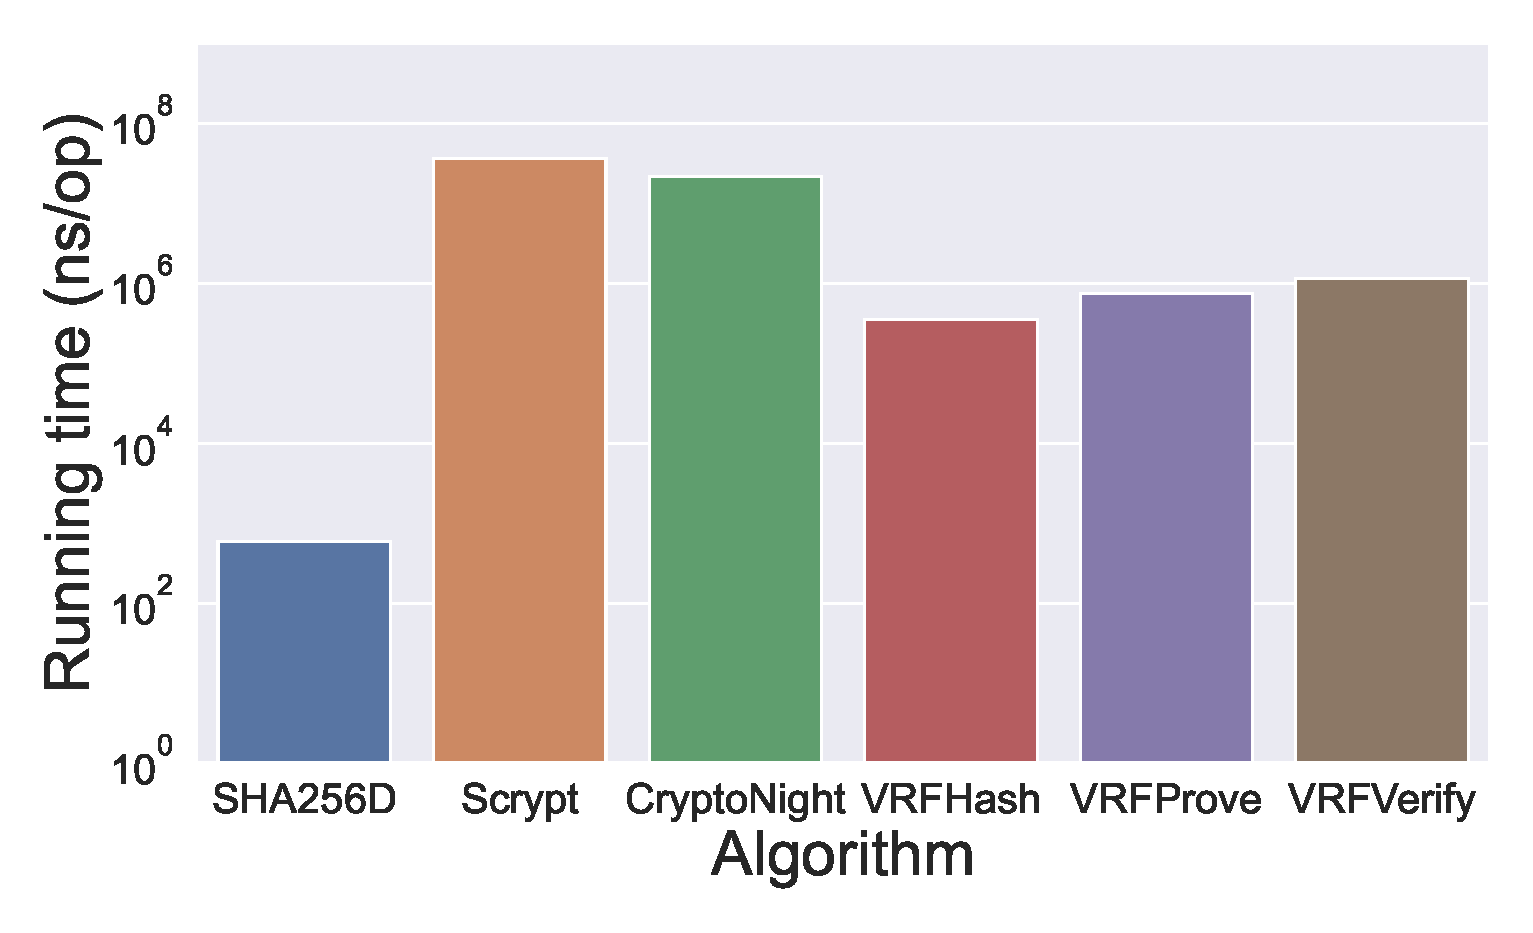
\includegraphics[width=.45\linewidth]{figs/runtime-comparison.eps}
        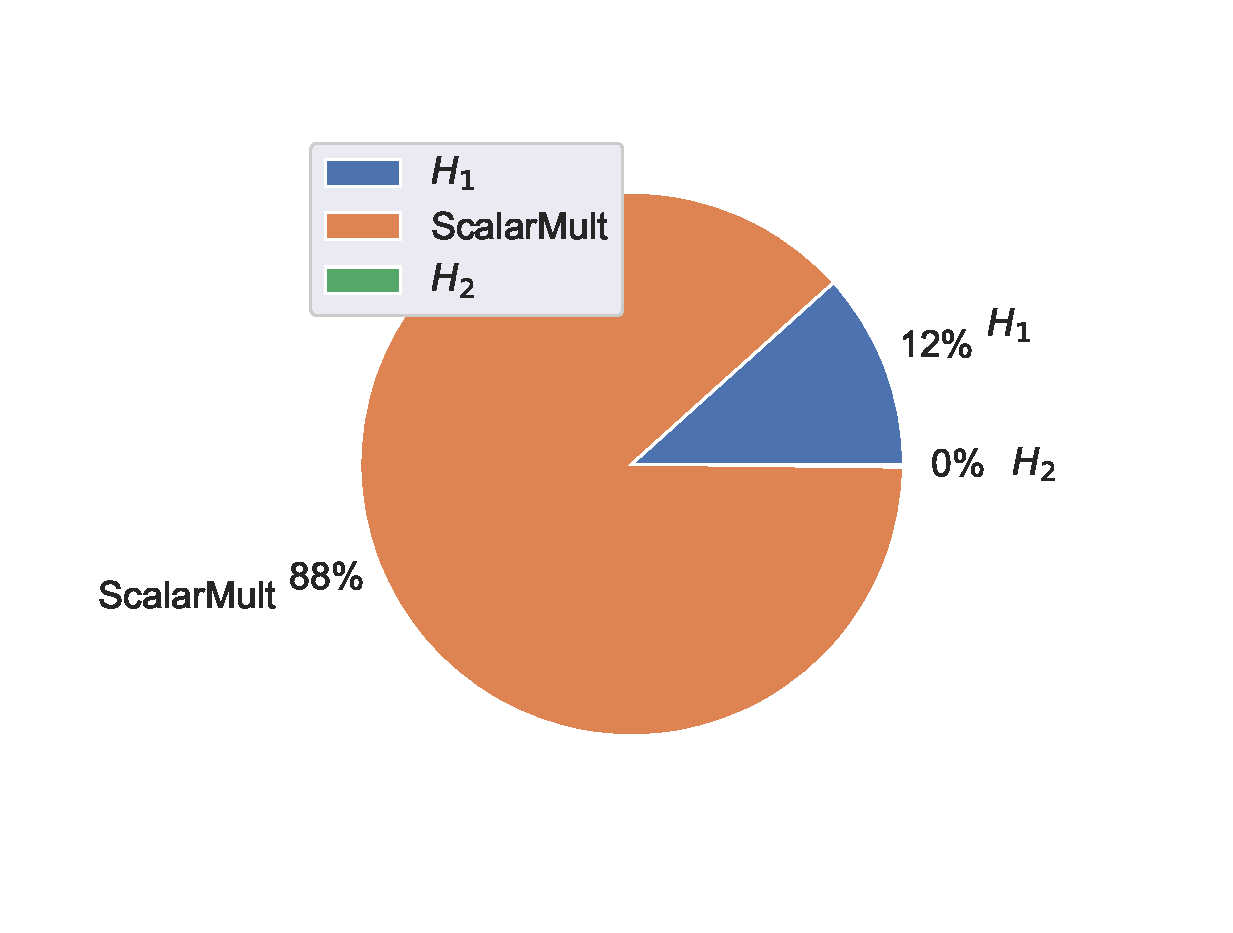
\includegraphics[width=.45\linewidth]{figs/runtime-breakdown.eps}
        \captionof{figure}{\color{Green} Runtime and profiling of VRFs.}
    \end{center}\vspace{1cm}


    \section*{Comparison with other solutions}

    To the best of our knowledge, VRF-based mining is the first construction that makes pooled mining \textit{impossible}.
    In this section, we briefly review related research on preventing mining pools, and compare them with VRF-based mining.
    We classify related research to two types, namely mining protocols trying to address pooled mining, and decentralised mining pools.

    \begin{center}
        \captionof{table}{\color{Green} Comparison between mining protocols.}
        \begin{tabular}{ccccc}
            \hline
                                          & VRF-based mining & Puzzle-1~\cite{miller2015nonoutsourceable} & Puzzle-2~\cite{miller2015nonoutsourceable} & 2P-PoW~\cite{2P-PoW} \\ \hline
            Punishment                    & New reward       & New reward                                 & New reward                                 & New reward           \\
            Stealing                      & Unlinkable       & Linkable                                   & Unlinkable                                 & Unlinkable           \\
            No partial outsourcing        & \cmark           & \cmark                                     & \cmark                                     & \xmark               \\
            Support randomised signatures & \cmark           & \cmark                                     & \cmark                                     & \xmark               \\
            No complex cryptography       & \cmark           & \cmark                                     & \xmark                                     & \cmark               \\ \hline
        \end{tabular}
    \end{center}

    \begin{center}
        \captionof{table}{\color{Green} Comparison with decentralised mining pools.}
        \begin{tabular}{ccccc}
            \hline
                             & VRF-based mining & P2Pool~\cite{voight2011p2pool} & SmartPool~\cite{luu2017smartpool} & BetterHash~\cite{draft-bip-BetterHash} \\ \hline
            Complexity       & -                & Blockchain                     & Smart contract                    & -                                      \\
            Decentralisation & Mining           & Mining                         & Mining                            & Select txs                             \\ \hline
        \end{tabular}
    \end{center}


    \section*{Conclusion and future work}

    We have proposed VRF-based mining, that can make pooled mining in Proof-of-work-based consensus impossible.
    VRF-based mining is simple and intuitive: Miners produce hashes of blocks using VRFs rather than hash functions, so a pool operator should reveal his private key to outsource the mining process to other miners.

    As aforementioned, ruling out pooled mining can achieve better decentralisation but may harm the incentive of mining.
    How to achieve decentralisation while preserving the incentive of mining is still an open challenge.

    %----------------------------------------------------------------------------------------
    %	REFERENCES
    %----------------------------------------------------------------------------------------

    % \nocite{*} % Print all references regardless of whether they were cited in the poster or not
    \bibliographystyle{plain} % Plain referencing style
    \bibliography{refs} % Use the example bibliography file sample.bib

    %----------------------------------------------------------------------------------------
    %	ACKNOWLEDGEMENTS
    %----------------------------------------------------------------------------------------

    \section*{Acknowledgements}

    We thank Cheng Wang, Omer Shlomovits and John Tromp for their valuable feedback.

    %----------------------------------------------------------------------------------------

\end{multicols}
\end{document}